\documentclass[12pt]{article}

\title{Newtonian gravitation from scratch, for C++ programmers}
\author{S. Halayka\footnote{sjhalayka@gmail.com}}
\date{\today\;\currenttime}

\usepackage{datetime}
\usepackage{listings}
\usepackage{cite}
\usepackage{xcolor}
\usepackage{graphicx}
\usepackage{setspace}
\usepackage{amsmath}
\usepackage{url}
\usepackage[margin=0.8in]{geometry}
\usepackage{listings}


\usepackage{xcolor}
\lstset { %
    language=C++,
    backgroundcolor=\color{black!5}, % set backgroundcolor
    basicstyle=\footnotesize,% basic font setting
    showstringspaces=false,
}


%\doublespace

%\usepackage[]{lineno}
%\linenumbers


\begin{document}



 
\maketitle

\begin{abstract}
This paper contains a short introduction to Newtonian gravitation.
The main focus is on some C++ code.
\end{abstract}




\section{Introduction}

In this paper, we cover the following seven subjects:
\begin{enumerate}
\item Typedefs that can be used to specify the precision of the floating point variables.
\item A custom 3D vector class that is used to encapsulate the data and member functions using object-oriented paradigms.
\item Some constants that are used throughout the paper.
\item A brute force integer field line intersection count function.
\item A heuristic real field line intersection count function.
\item An application is demonstrated, where we model Mercury's orbit by using numerical integration.
A full code is given.
\item Conclusion: general relativity versus Newtonian gravitation.
\end{enumerate}

The main goal is to acquaint the coder with the basic mathematics behind Mercury's orbit due to Newtonian gravitation.

The following two assumptions are made:
\begin{enumerate}
\item Like with the irradiance of light (e.g. WiFi strength) and the intensity of sound, we assume in this paper that the acceleration in Newton's gravity follows an inverse-square law:
\begin{equation}
g_N \propto \frac{1}{R^2}.
\end{equation}
See Fig. 1.
\begin{figure} 
\centering
  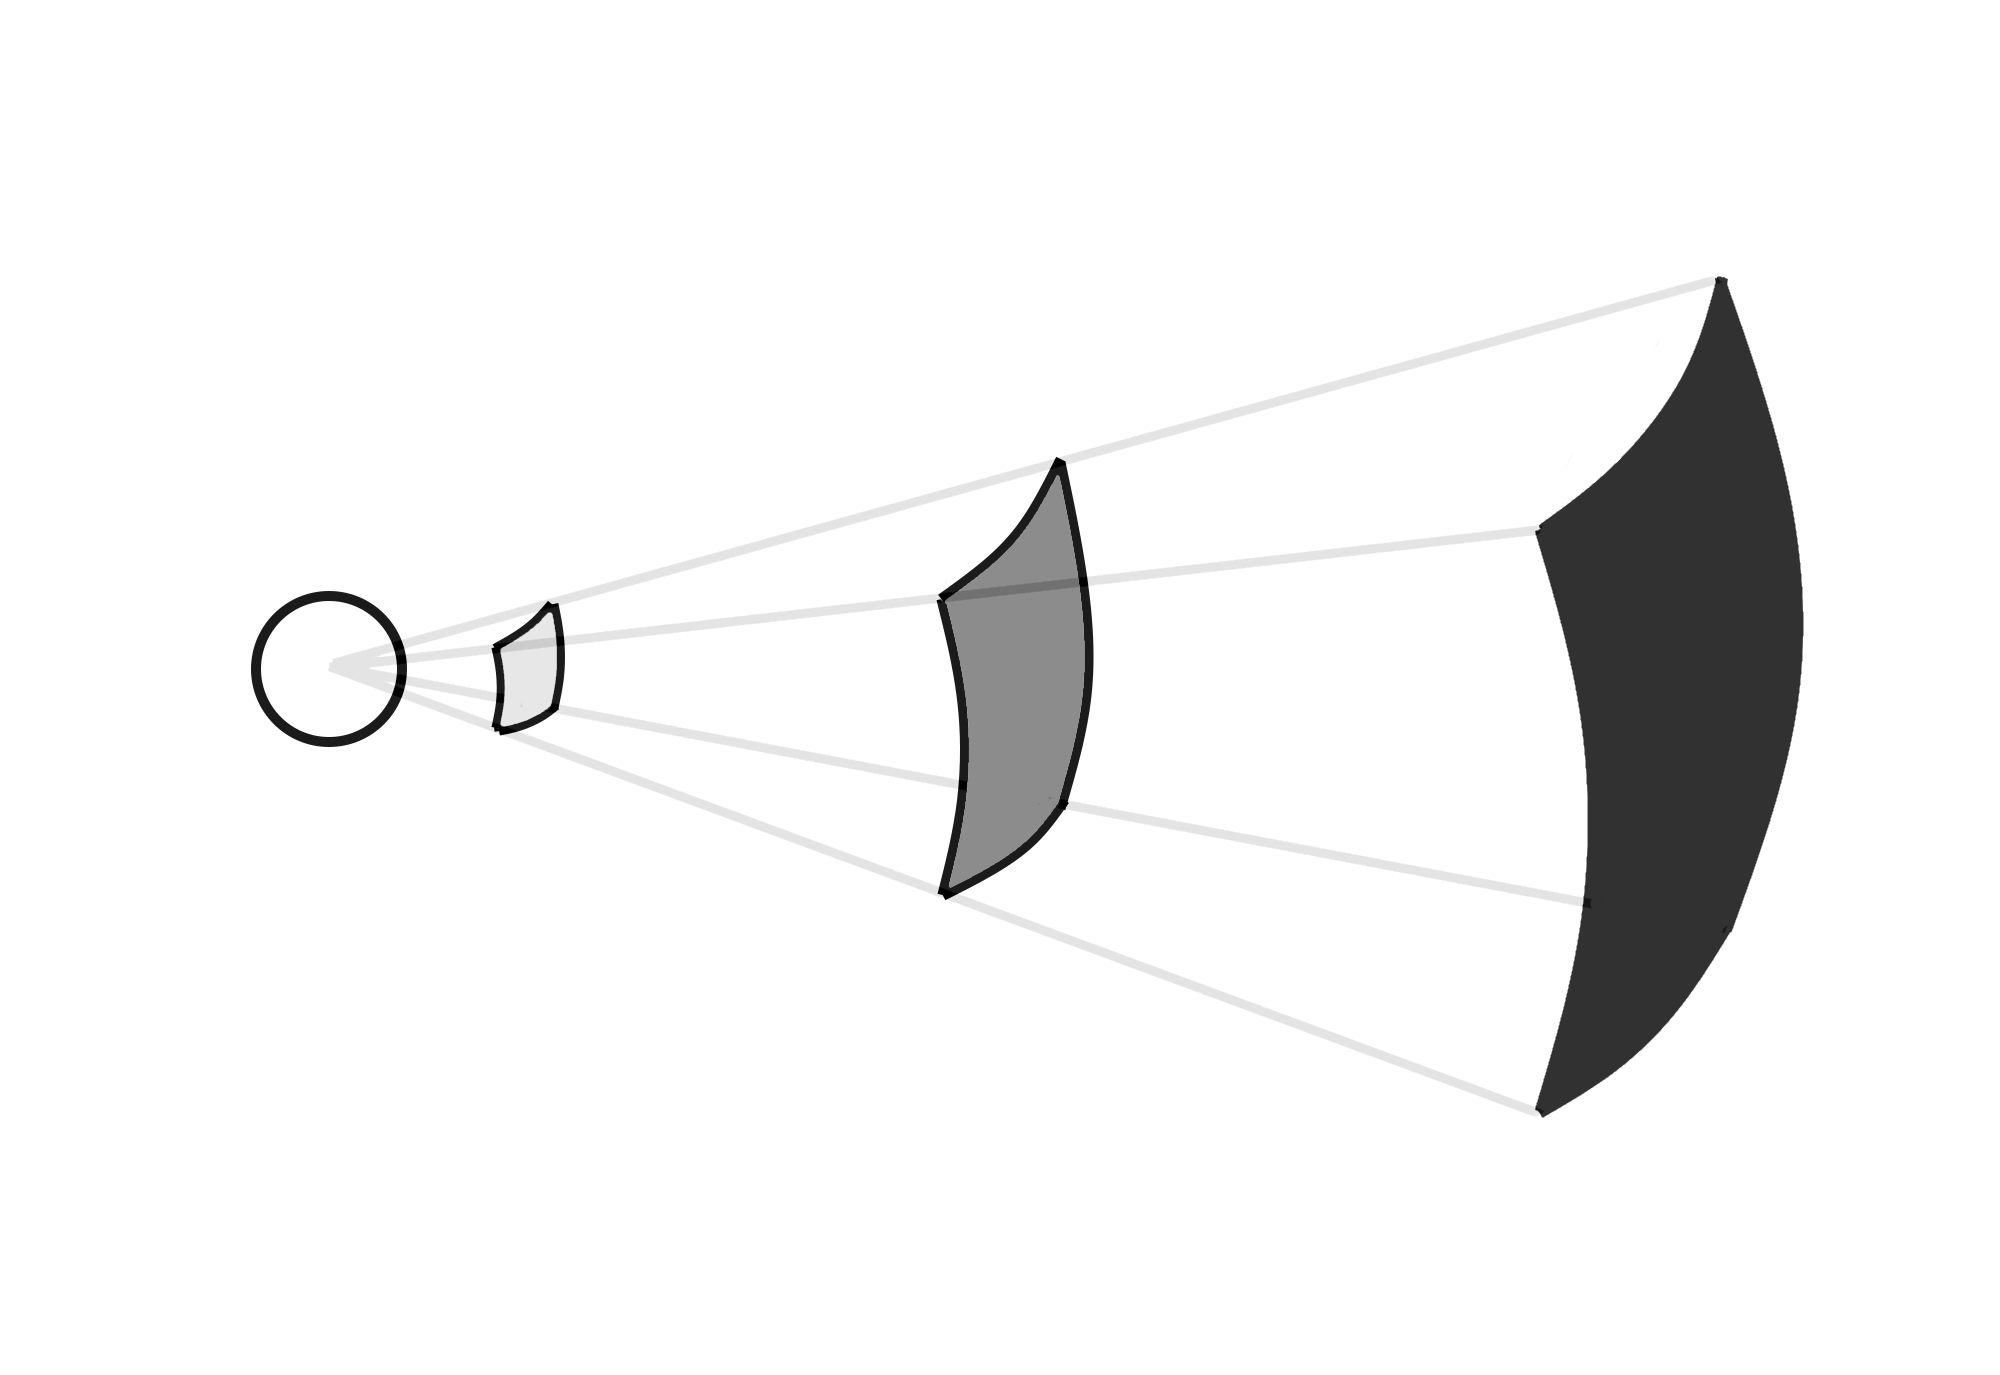
\includegraphics[width = 5 in]{inverse_square_law.png}
  \caption{
Inverse-square law visualized.
The gravitational acceleration is $g_N \propto 1/R^2$.
}
\end{figure}

\item The other assumption that we make in this paper is that the gravitational field line count is given by the holographic principle \cite{hooft, susskind}, for lack of a better method.
\end{enumerate}





\section{Typedefs}
In this tutorial, we leave the real number type up to the coder.
For instance, we can use quad-precision long doubles (e.g. 16-byte floating point variables on Ubuntu):
\begin{lstlisting}
typedef long double real_type;
\end{lstlisting}
On the other hand, we can use the Boost multiprecision library just as easily.
Here we can use oct-precision variables (e.g. 32-byte floating point variables on all platforms):
\begin{lstlisting}
#include <boost/multiprecision/cpp_bin_float.hpp>
using namespace boost::multiprecision;

typedef number<
	backends::cpp_bin_float<
		237,
		backends::digit_base_2, 
		void, 
		std::int32_t, 
		-262142, // 2^18 == 262144
		262143>, 
	et_off> cpp_bin_float_oct;

	// 237 significand bits
	// + 18 exponent bits 
	// + 1 sign bit = 
	// 256 bits (32 bytes)

typedef cpp_bin_float_oct real_type;
\end{lstlisting}





\section{Custom 3D vector class}
The tutorial also makes use of a 3D vector class:
\begin{lstlisting}
class vector_3
{
public:
	real_type x, y, z;

	// Overloaded operators go here

	real_type dot(const vector_3& rhs) const
	{
		return x*rhs.x + y*rhs.y + z*rhs.z;
	}

	real_type self_dot(void) const
	{
		return x*x + y*y + z*z;
	}

	real_type length(void) const
	{
		return sqrt(self_dot());
	}

	vector_3& normalize(void)
	{
		const real_type len = length();

		if(len != 0)
		{
			x /= len;
			y /= len;
			z /= len;
		}

		return *this;
	}
};
\end{lstlisting}




\section{Constants}

The following constants will be used in this tutorial:
\begin{lstlisting}
const real_type pi = 4.0 * atan(1.0);
const real_type G = 6.67430e-11; // Newton's constant
const real_type c = 299792458; // Speed of light in vacuum
const real_type c2 = c * c;
const real_type c3 = c * c * c;
const real_type c4 = c * c * c * c;
const real_type h = 6.62607015e-34; // Planck's constant
const real_type hbar = h / (2.0 * pi);
const real_type k = 1.380649e-23; // Boltzmann's constant
\end{lstlisting}



\section{Brute force: integer field line count}

The main idea behind this tutorial is that there is a finite number of field lines extending out from a gravitating body.
See Fig. 2.
\begin{figure} 
\centering
  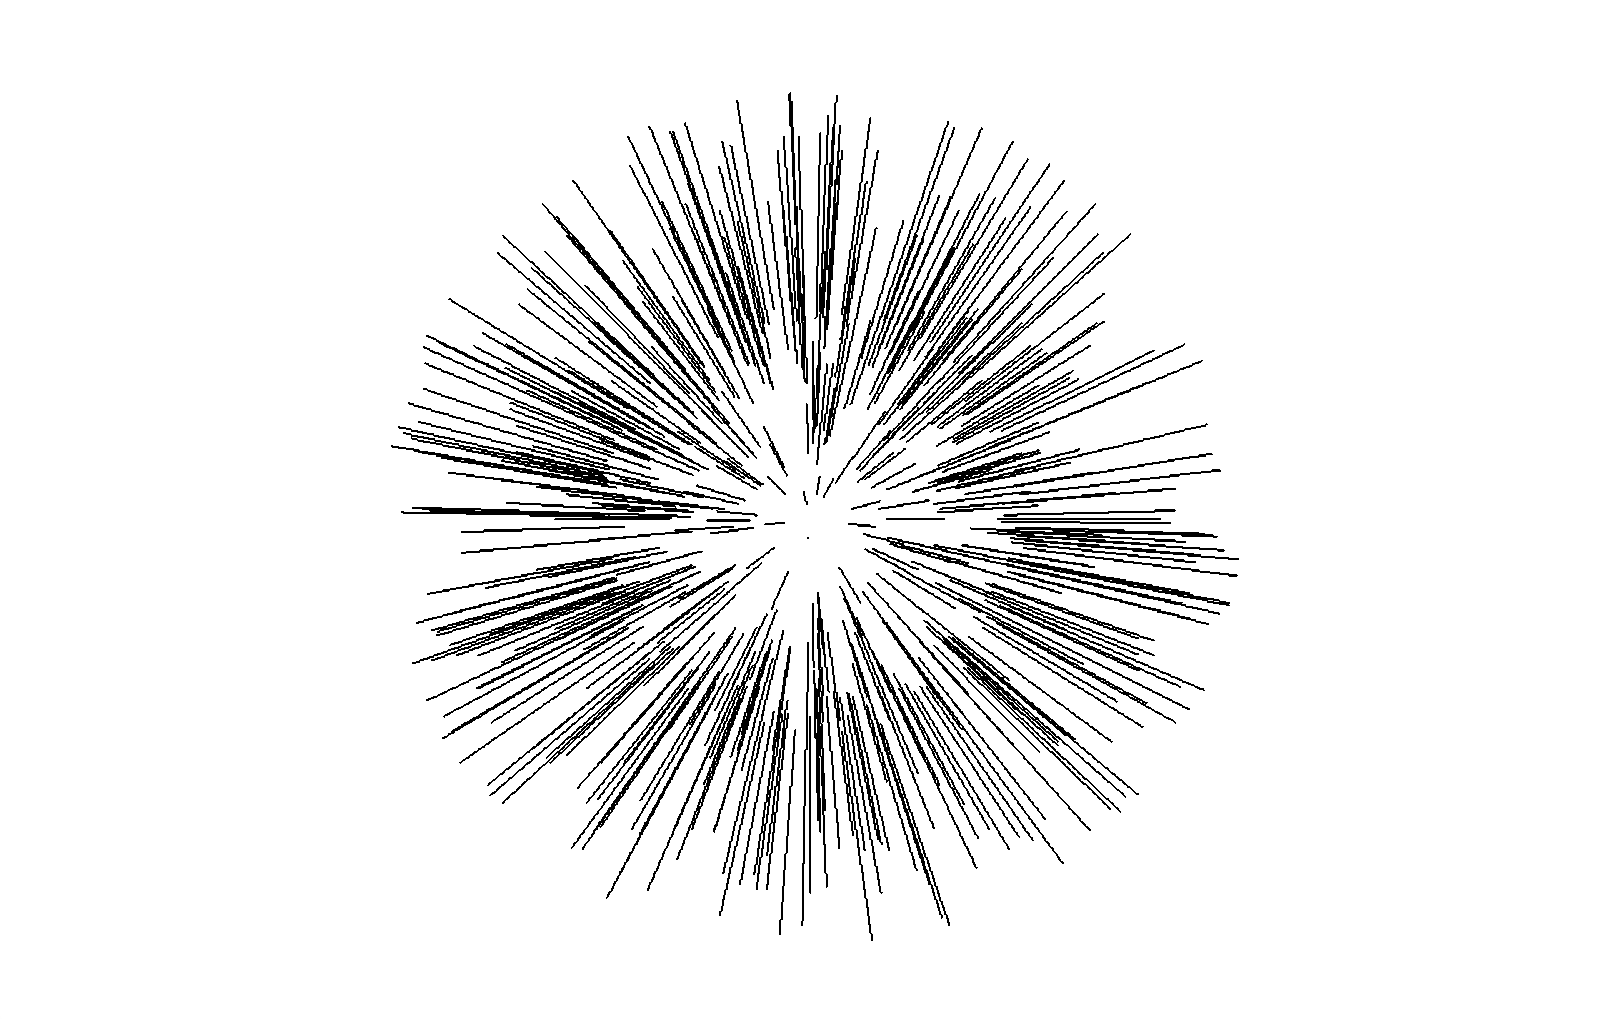
\includegraphics[width = 3 in]{3.png}
  \caption{
The emitter is spherical.
The field line starting positions are placed pseudorandomly on a 2-sphere, and the normals (e.g. field line directions) are calculated using the same positions.
}
\end{figure}

We use the field line intersection count to signify field strength, from which we can obtain the gradient.

Where $r$ is the receiver radius, $R$ is the distance from the centre of the emitter, $\beta$ is the get intersecting line count function, and $n$ is the field line count, the gradient (e.g. directional derivative) is:
\begin{equation}
\alpha = \frac{\beta(R + \epsilon) - \beta(R)}{\epsilon}.
\end{equation}
The gradient strength is:
\begin{equation}
g = \frac{-\alpha}{r^2}.
\end{equation}

\begin{lstlisting}
long long unsigned int get_intersecting_line_count(
	const vector<vector_3>& unit_vectors,
	const vector_3& sphere_location,
	const real_type sphere_radius)
{
	long long unsigned int count = 0;

	// Get cross-section edge direction
	vector_3 cross_section_edge_dir(sphere_location.x, sphere_radius, 0);
	cross_section_edge_dir.normalize();

	// Get receiver direction
	vector_3 receiver_dir(sphere_location.x, 0, 0);
	receiver_dir.normalize();

	// The minimum threshold for intersection
	const real_type min_dot = cross_section_edge_dir.dot(receiver_dir);

	for (size_t i = 0; i < unit_vectors.size(); i++)
		if (unit_vectors[i].dot(receiver_dir) >= min_dot)
			count++; // Intersection occurred

	return count;
}
\end{lstlisting}

\begin{lstlisting}
int main(int argc, char** argv)
{
	// Field line count
	const size_t n = 1000000000;

	cout << "Allocating memory for field lines" << endl;
	vector<vector_3> unit_vectors(n);

	for (size_t i = 0; i < n; i++)
	{
		unit_vectors[i] = pseudorandom_unit_vector();

		static const size_t output_mod = 10000;

		if (i % output_mod == 0)
			cout << "Getting pseudorandom locations: " 
			<< static_cast<float>(i) / n << endl;
	}

	string filename = "newton.txt";
	ofstream out_file(filename.c_str());
	out_file << setprecision(30);

	const real_type start_distance = 10.0;
	const real_type end_distance = 100.0;
	const size_t distance_res = 1000;

	const real_type distance_step_size = 
		(end_distance - start_distance) 
		/ (distance_res - 1);

	for (size_t step_index = 0; step_index < distance_res; step_index++)
	{
		const real_type r = 
			start_distance + 
			step_index * distance_step_size;

		const vector_3 receiver_pos(r, 0, 0);
		const real_type receiver_radius = 1.0;

		const real_type epsilon = 1.0;

		vector_3 receiver_pos_plus = receiver_pos;
		receiver_pos_plus.x += epsilon;

		const long long signed int collision_count_plus = 
			get_intersecting_line_count(
				unit_vectors, 
				receiver_pos_plus, 
				receiver_radius);
		
		const long long signed int collision_count = 
			get_intersecting_line_count(
				unit_vectors, 
				receiver_pos, 
				receiver_radius);
		
		const real_type gradient = 
			static_cast<real_type>
			(collision_count_plus - collision_count) 
			/ epsilon;
		
		const real_type gradient_strength = 
			-gradient 
			/ (receiver_radius * receiver_radius);

		cout << "r: " << r << " gradient strength: " 
		<< gradient_strength << endl;

		out_file << r << " " << gradient_strength << endl;
	}

	out_file.close();

	return 0;
}
\end{lstlisting}

While this method works, it is both memory and processor intensive.
This method is meant to be a stepping stone for the next section.







\section{Heuristic: real field line count}

Rather than allocating gigabytes of RAM to store some unit vectors, we can instead use a heuristic approach to solve the problem from the previous section.
This heuristic solution instead uses basic geometry to obtain the intersection count.

Where $r$ is the receiver radius, $R$ is the distance from the centre of the emitter, $\beta$ is the get intersecting line count function, and $n$ is the field line count, the gradient is:
\begin{equation}
\alpha = \frac{\beta(R + \epsilon) - \beta(R)}{\epsilon}.
\end{equation}

Here we assume that the number of field lines is given by the holographic principle:
\begin{equation}
n = \frac{A k c^3}{ 4 G \hbar \log 2}.
\end{equation}

The gradient strength is:
\begin{equation}
g = \frac{-\alpha}{r^2} \approx \frac{n}{2 R^3}.
\end{equation}
From this we can get the Newtonian gradient, in terms of either $n$, $g$, $A$, or $G M$:
\begin{equation}
\label{g_N_equation}
g_N = \frac{n c \hbar \log 2}{k 4 \pi M R^2} = \frac{g R c \hbar \log 2}{k 2 \pi M} = \frac{A c^4}{16 \pi G M R^2} = \frac{G M}{R^2}.
\end{equation}

We will use $g_N = {G M}/{R^2}$, the simplest version of $g_N$, in the next section.

\begin{lstlisting}
real_type get_intersecting_line_count(
	const real_type n,
	const vector_3& sphere_location,
	const real_type sphere_radius)
{
	const real_type sphere_area = 
		4 * pi * sphere_location.x * sphere_location.x;

	const real_type circle_area = 
		pi * sphere_radius * sphere_radius;
	
	const real_type ratio = 
		circle_area / sphere_area;
	
	return n * ratio;
}
\end{lstlisting}

\begin{lstlisting}
int main(int argc, char** argv)
{
	const real_type emitter_radius = 1.0;
	
	const real_type emitter_area = 
		4.0 * pi * emitter_radius * emitter_radius;

	// Field line count
	// re: holographic principle:
	const real_type n = 
		(k * c3 * emitter_area) 
		/ (log(2.0) * 4.0 * G * hbar);

	const real_type emitter_mass = c2 * emitter_radius / (2.0 * G);

	// 2.39545e47 is the 't Hooft-Susskind constant:
	// the number of field lines for a black hole of
	// unit Schwarzschild radius
	//
	//const real_type G_ = 
	//	(k * c3 * pi) 
	//	/ (log(2.0) * hbar * 2.39545e47);

	const string filename = "newton.txt";
	ofstream out_file(filename.c_str());
	out_file << setprecision(30);

	const real_type start_distance = 10.0;
	const real_type end_distance = 100.0;
	const size_t distance_res = 1000;

	const real_type distance_step_size =
		(end_distance - start_distance)
		/ (distance_res - 1);

	for (size_t step_index = 0; step_index < distance_res; step_index++)
	{
		const real_type r =
			start_distance + step_index * distance_step_size;

		const vector_3 receiver_pos(r, 0, 0);
		const real_type receiver_radius = 1.0;

		const real_type epsilon = 1.0;

		vector_3 receiver_pos_plus = receiver_pos;
		receiver_pos_plus.x += epsilon;

		const real_type collision_count_plus =
			get_intersecting_line_count(
				n,
				receiver_pos_plus,
				receiver_radius);

		const real_type collision_count =
			get_intersecting_line_count(
				n,
				receiver_pos,
				receiver_radius);

		const real_type gradient =
			(collision_count_plus - collision_count)
			/ epsilon;

		real_type gradient_strength =
			-gradient
			/ (receiver_radius * receiver_radius);

		const real_type gradient_strength_ = 
			n / (2.0 * pow(receiver_pos.x, 3.0));

		const real_type newton_strength = 
			n * c * hbar * log(2.0)
			/ 
			(k * pow(receiver_pos.x, 2.0) 
				* emitter_mass * 4.0 * pi);

		const real_type newton_strength_ =
			G * emitter_mass / pow(receiver_pos.x, 2.0);

		cout << "r: " << r << " gradient strength: "
			<< gradient_strength << endl;

		out_file << r << " " << gradient_strength << endl;
	}

	out_file.close();

	return 0;
}
\end{lstlisting}

This method is faster and less memory intensive when compared to the integer field count method.
This method is meant to be a stepping stone for the next section.

For reference, if you know $n$, and you wish to know the emitter radius from that, then the equation is:
\begin{equation}
r_{\textit{emitter}} = \sqrt{\frac{n G \hbar \log 2}{k c^3 \pi}}.
\end{equation}
Using this radius, one can ensure that the results from this section match the results of the previous section, where $n$ is relatively small anyway (e.g. $n = 10^7$).
As for predictability, for instance where $n = 10^7$ (e.g. $r_{\textit{emitter}} = 6.46109 \times 10^{-21}$ metres), it is found that at a distance of $170.521$ metres that the gradient $-\alpha = 0.999615$ dips below $1.0$.
This distance value depends entirely on our use of the holographic principle.




\section{Application: modeling Mercury's orbit using numerical integration}

In essence, the numerical calculation of the Newtonian orbit of Mercury is as follows:
\begin{enumerate}
\item Place Mercury at the aphelion to start.
\item Calculate the orbit path by repeatedly taking steps in time.
\end{enumerate}

The constant time step is:
\begin{lstlisting}
const real type dt = 10000; // 2.77777 hours
\end{lstlisting}

The initial conditions are:
\begin{lstlisting}
vector_3 Mercury_pos(0, 69817079000.0, 0); // Aphelion location
vector_3 Mercury_vel(-38860, 0, 0); // Aphelion velocity
\end{lstlisting}

The orbit code is as follows. 
Here we use Eq. \ref{g_N_equation} (e.g. $g_N = {G M}/{R^2}$) to calculate the acceleration from Newtonian gravitation:
\begin{lstlisting}
vector_3 Newtonian_acceleration(
	const real_type emitter_mass,
	const vector_3& pos, // Receiver pos
	const real_type G)
{
	// Sun's position is fixed at the origin
	vector_3 grav_dir = vector_3(0, 0, 0) - pos;
	const real_type distance = grav_dir.length();
	grav_dir.normalize();

	vector_3 accel = grav_dir * G * emitter_mass / pow(distance, 2.0);

	return accel;
}
\end{lstlisting}

Here we show the Euler integration, which is extremely simple.
The acceleration is calculated, then it is added (e.g. integrated) to the velocity.
Once that's done, the velocity is added to the position.
See Figs. 3 and 4.
\begin{figure} 
\centering
\label{fig3}
  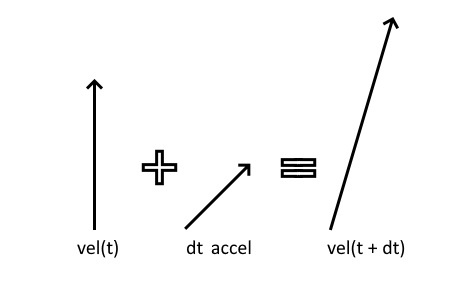
\includegraphics[width = 4 in]{velocity.png}
  \caption{
A diagram of the Euler integration of velocity.
}
\end{figure}
\begin{figure} 
\centering
\label{fig4}
  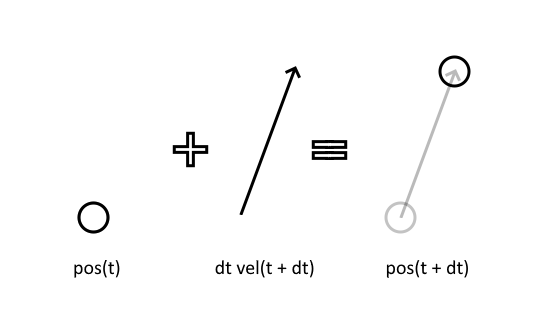
\includegraphics[width = 4 in]{position.png}
  \caption{
A diagram of the Euler integration of position.
}
\end{figure}

\begin{lstlisting}
void proceed_Euler(
	vector_3& pos, 
	vector_3& vel, 
	const real_type G, 
	const real_type dt)
{
	vector_3 accel = 
		Newtonian_acceleration(
			emitter_mass, 
			pos, 
			G);

	vel += accel * dt;
	pos += vel * dt;
}

\end{lstlisting}

The passage of time is computed whenever the window manager (e.g. OpenGL/GLUT) is not busy drawing or processing input:
\begin{lstlisting}
void idle_func(void)
{
	proceed_Euler(Mercury_pos, Mercury_vel, G, dt);
}
\end{lstlisting}

On the other hand, rather than using Euler integration, the 4th-order symplectic integration does a better job at conserving energy, but at a speed cost:
\begin{lstlisting}
void proceed_symplectic_order_4(
	vector_3& pos, 
	vector_3& vel, 
	real_type G, 
	real_type dt)
{
	static const real_type cr2 = 
		pow(2.0, 1.0 / 3.0);

	static const real_type c[4] =
	{
		1.0 / (2.0 * (2.0 - cr2)),
		(1.0 - cr2) / (2.0 * (2.0 - cr2)),
		(1.0 - cr2) / (2.0 * (2.0 - cr2)),
		1.0 / (2.0 * (2.0 - cr2))
	};

	static const real_type d[4] =
	{
		1.0 / (2.0 - cr2),
		-cr2 / (2.0 - cr2),
		1.0 / (2.0 - cr2),
		0.0
	};

	pos += vel * c[0] * dt;
	vel += Newtonian_acceleration(
			emitter_mass, 
			pos, 
			G) * d[0] * dt;

	pos += vel * c[1] * dt;
	vel += Newtonian_acceleration(
			emitter_mass, 
			pos, 
			G) * d[1] * dt;

	pos += vel * c[2] * dt;
	vel += Newtonian_acceleration(
			emitter_mass, 
			pos, 
			G) * d[2] * dt;

	pos += vel * c[3] * dt;
	// last element d[3] is always 0
}
\end{lstlisting}

See Fig. 5.
\begin{figure} 
\centering
  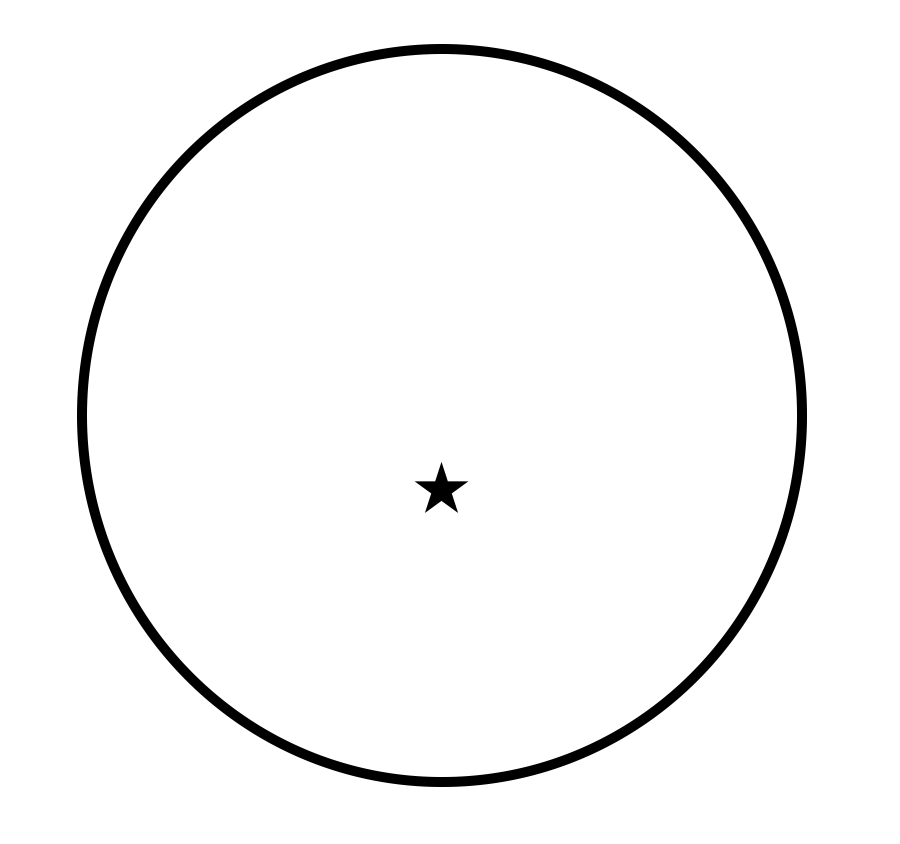
\includegraphics[width = 4 in]{mercury.png}
  \caption{
Mercury in orbit around the Sun.
Note that the orbit path is slightly elliptical.
}
\end{figure}

A full code, which models the orbit of Mercury, is at:

\url{https://github.com/sjhalayka/mercury_orbit_glut}






\section{Conclusion: general relativity versus Newtonian gravitation}

In Newtonian gravity, the isotropic emitter ensures that space is curved.
This is not quite the same as what happens in general relativity \cite{misner}.
In general relativity, time is also curved.
One way to try to model the curvature of time is to produce graviton overlap by using pseudorandom direction vectors.
These matters will be the focus of a future tutorial.



%In order to compensate for this, one can convert the field lines into field cylinders.
%The overlap of the cylinders only occurs if the cylinder radii are larger than the Planck scale.
%This overlap would have to be useful, somehow, for calculating the gravitational time dilation $d\tau/dt = \sqrt{1 - r_{\textit{emitter}}/R}$.
%This overlap essentially requires that the gravitons have spatial extent no smaller than the Planck scale; not point-like.











\begin{thebibliography}{9}

\bibitem{hooft} `t Hooft. Dimensional reduction in quantum gravity. (1993)
\bibitem{susskind} Susskind. The World as a Hologram. (1994)
\bibitem{misner} Misner et al. Gravitation. (1970)

%\bibitem{fiedler1} Fiedler. Fix Your Timestep! (2004)
%\bibitem{fiedler2} Fiedler. Integration Basics. (2004)
%\bibitem{nasa} Williams. NASA Mercury Fact Sheet. (2024)



\end{thebibliography}














\end{document}









